\item \points{4h} \textbf{Implicit regularization of batch size}

We still work with the setup in part (e). For this sub-question, we use the same dataset and starter code as in sub-question (f). We will show that the noise in the training process also induces implicit regularization. In particular, the noise introduced by \emph{stochastic} gradient descent in this case helps generalization. \textbf{Implement} the SGD algorithm in the \texttt{QP.train\_SGD} function and run it with batch size $\{1, 5, 40\}$, learning rate $0.08$, and initialization $\alpha=0.1$. For simplicity, the code for selecting a batch of examples is already provided in the starter code.

Your generated plot should like like the following:

\begin{figure}[H]
    \centering
    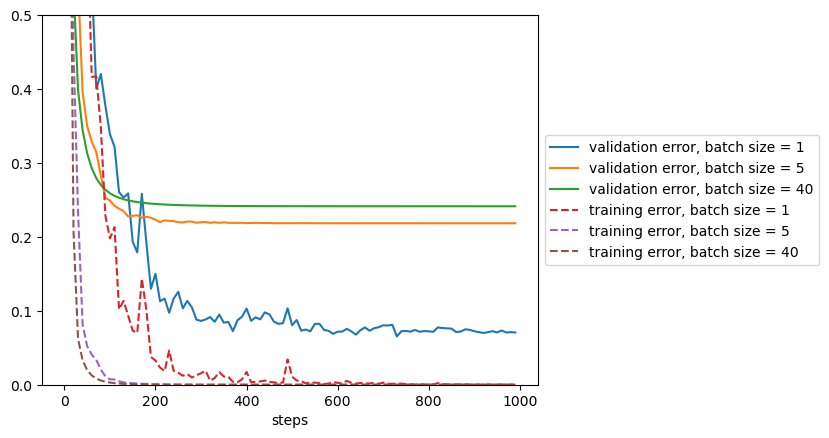
\includegraphics[width=.7\linewidth]{04-implicitreg/implicitreg_quadratic_batchsize.png}
\end{figure}

The plot shows that the stochasticity in the training process is also an important factor in the generalization performance --- in our setting, SGD finds a solution that generalizes better. In fact, a conjecture is that stochasticity in the optimization process (such as the noise introduced by a small batch size) helps the optimizer to find a solution that generalizes better. This conjecture can be proved in some simplified cases, such as the quadratically parameterized model in this sub-question (adapted from the paper \href{https://arxiv.org/abs/2006.08680}{HaoChen et al., 2020}), and can be observed empirically in many other cases.

\textbf{Files to Submit: }\texttt{src-implicitreg/submission.py}